% This document is based on a template created by Ted Pavlic (http://www.tedpavlic.com)


%----------------------------------------------------------------------------------------
%	PACKAGES AND OTHER DOCUMENT CONFIGURATIONS
%----------------------------------------------------------------------------------------

\documentclass{article}

\usepackage{fancyhdr} % Required for custom headers
\usepackage{lastpage} % Required to determine the last page for the footer
\usepackage{extramarks} % Required for headers and footers
\usepackage[usenames,dvipsnames]{color} % Required for custom colors
\usepackage{graphicx} % Required to insert images
\usepackage{subcaption}
\usepackage{listings} % Required for insertion of code
\usepackage{courier} % Required for the courier font
%\usepackage{lipsum} % Used for inserting dummy 'Lorem ipsum' text into the template
\usepackage{amsmath,siunitx,physics,amssymb}
\usepackage{placeins}
\usepackage{enumitem}
\usepackage{animate}
\usepackage[backend=biber,style=ieee]{biblatex}
\usepackage{hyperref,cleveref}

\addbibresource{deepviz.bib}

% Margins
\topmargin=-0.45in
\evensidemargin=0in
\oddsidemargin=0in
\textwidth=6.5in
\textheight=9.0in
\headsep=0.25in

\linespread{1.1} % Line spacing

% Set up the header and footer
\pagestyle{fancy}
\lhead{\hmwkAuthorName} % Top left header
\chead{\hmwkClass\ (\hmwkClassTime): \hmwkTitle} % Top center head
%\rhead{\firstxmark} % Top right header
\lfoot{\lastxmark} % Bottom left footer
\cfoot{} % Bottom center footer
\rfoot{Page\ \thepage\ of\ \protect\pageref{LastPage}} % Bottom right footer
\renewcommand\headrulewidth{0.4pt} % Size of the header rule
\renewcommand\footrulewidth{0.4pt} % Size of the footer rule

%\setlength\parindent{0pt} % Removes all indentation from paragraphs

%----------------------------------------------------------------------------------------
%	DOCUMENT STRUCTURE COMMANDS
%	Skip this unless you know what you're doing
%----------------------------------------------------------------------------------------

% Header and footer for when a page split occurs within a problem environment
\newcommand{\enterproblemHeader}[1]{
%\nobreak\extramarks{#1}{#1 continued on next page\ldots}\nobreak
%\nobreak\extramarks{#1 (continued)}{#1 continued on next page\ldots}\nobreak
}

% Header and footer for when a page split occurs between problem environments
\newcommand{\exitproblemHeader}[1]{
%\nobreak\extramarks{#1 (continued)}{#1 continued on next page\ldots}\nobreak
%\nobreak\extramarks{#1}{}\nobreak
}

\newcommand{\numberthis}{\addtocounter{equation}{1}\tag{\theequation}}

%----------------------------------------------------------------------------------------
%	NAME AND CLASS SECTION
%----------------------------------------------------------------------------------------

\newcommand{\hmwkTitle}{Assignment\ \#$2$ Bonus} % Assignment title
\newcommand{\hmwkDueDate}{Friday,\ February\ 26,\ 2018} % Due date
\newcommand{\hmwkClass}{CSC411} % Course/class
\newcommand{\hmwkClassTime}{L2001} % Class/lecture time
\newcommand{\hmwkAuthorName}{Lukas Zhornyak} % Your name

%----------------------------------------------------------------------------------------
%	TITLE PAGE
%----------------------------------------------------------------------------------------

\title{
	\vspace{2in}
	\textmd{\textbf{\hmwkClass:\ \hmwkTitle}}\\
	\normalsize\vspace{0.1in}\small{Due\ on\ \hmwkDueDate}\\
	\vspace{0.1in}
	\vspace{3in}
}

\author{\textbf{\hmwkAuthorName}}
%\date{} % Insert date here if you want it to appear below your name

%----------------------------------------------------------------------------------------

\begin{document}

\maketitle
\clearpage

%----------------------------------------------------------------------------------------
%	ENVIRONMENT
%----------------------------------------------------------------------------------------

\section{Environment}	
This submission was created with Python 3.6.4 with numpy 1.14.1, scipy 1.0.0, scikit-image 0.13.1, and matplotlib 2.1.2, pytorch 0.3.0, torchvision 0.2.0, opencv 3.3.1, as well as all associated dependencies. 

The various visualizations shown in \cref{sec:main} are produced with the help of the Convolutional Neural Network Visualizations repository created by Utku Ozbulak\footnote{Available from \url{https://github.com/utkuozbulak/pytorch-cnn-visualizations}}, use with permission under the MIT license. A slightly modified version of the code is included with this submission. Modifications were made to facilitate inclusion as a package in this submission and to facilitate use of a custom neural network model. 

All images used are 277 by 277 pixels\footnote{Odd size is due to misreading the typical size for AlexNet. I would expect all results to be extensible to different image sizes however.} from the same database used in Assignment 2.
\clearpage

\section{Warm-up}\label{sec:warm up}

The weights of the first layer of AlexNet are shown in \cref{fig:layer1 weight}. Each filter displays some sort of simple colour pattern, most commonly either stripes, boundaries, or single dots. The more complicated patterns also tend to be nearly black and white, suggesting a separation in the detections of colour boundaries and patterns. In either case, the majority of the patterns seem to be focused on some variety of edge detection, as might be expected from the first layer of a convolutional neural network (CNN).

\Cref{fig:layer1 activate} shows the regions in the available dataset the most activate their corresponding filter. A brief examination of the images reinforces the idea that the filter in this first layer are focused on edge detection since the majority of the images in \cref{fig:layer1 activate} show some sort of distinct boundary and/or line. \Cref{fig:layer1 activate border} provides context to these crops. Some notable repeats include glasses, mouths, and eyes, and the letter "W". It also seems that many of the crops come from a smaller subset of images, suggesting that there is an overlap in what the activates the different neurons.

\begin{figure}
	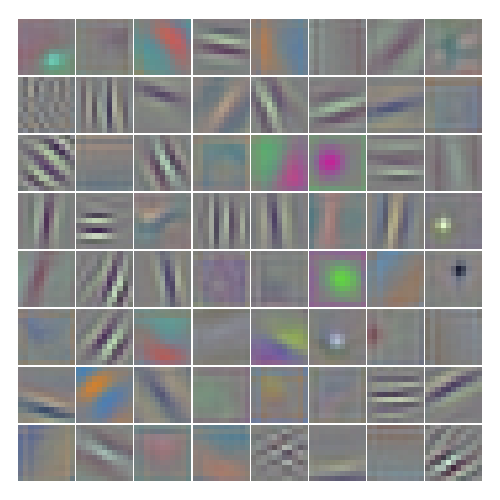
\includegraphics[width=\linewidth]{layer_1_weights}
	\caption{Visualization of the weights of the sixty-four \(11 \cross 11 \cross 3\) filters in the first layer of the pre-trained AlexNet, visualized in colour based on which colour channel the weights access.}
	\label{fig:layer1 weight}
\end{figure}
\begin{figure}
	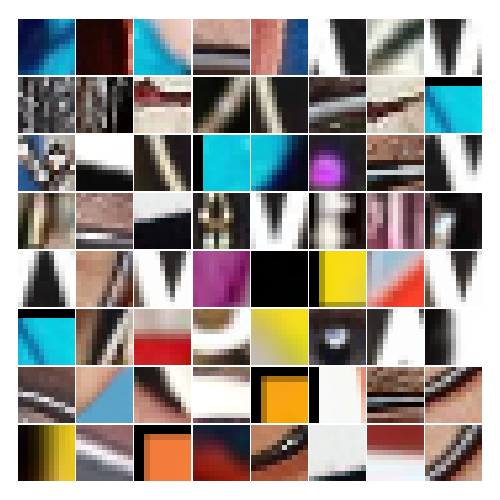
\includegraphics[width=\linewidth]{layer1_activate}
	\caption{Crop of the regions in the dataset which most activate the filters shown in \cref{fig:layer1 weight}.}
	\label{fig:layer1 activate}
\end{figure}
\begin{figure}
	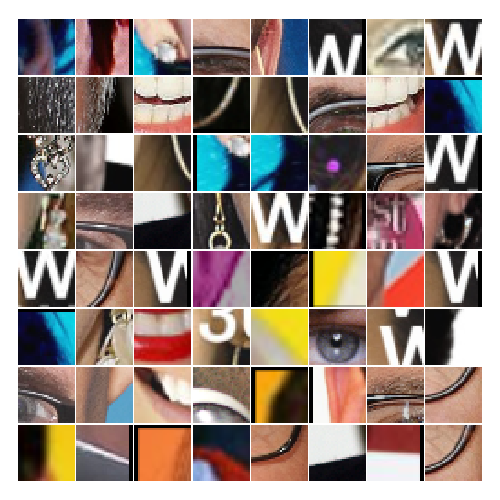
\includegraphics[width=\linewidth]{layer1_activate_border}
	\caption{Expanded view of the regions shown in \cref{fig:layer1 activate} to shown context of crop.}
	\label{fig:layer1 activate border}
\end{figure}

\clearpage

\FloatBarrier
\section[Visualization]{Visualizing the Deep Network}\label{sec:main}

In creating many of these visualization, a base image is needed. For this reason, the image associated with each actor that had the smallest loss against the expected label was selected. This can be interpreted as the image that the CNN is most confident is an image of the person. These images (\cref{fig:prototypical}) show clear, nearly head-on views of the person without any obstructing features. The case may be made to use the image the had the largest one-hot value for that label, as this in some ways represents what the CNN views as the "most" like the person.

The simplest way to visualize what a CNN views as the most important features is by simply visualizing the gradients produces from backpropagation. This is shown in the middle column of \cref{fig:vanilla backpropagation}. It is difficult to make out much from just these gradient, but if the results are normalized we get a saliency map (right column of \cref{fig:vanilla backpropagation}) that shows much more important features. The eyes and nose can be made out in several of these images, suggesting their importance in classification.

An improvement to backpropagation can be made by ignoring the negative gradients. In this way, only those features which given a positive contribution to the classification will be shown -- those features which given the impression of that person. This is shown, along with the saliency map, in \cref{fig:guided backpropagation}. Again, the importance of the eyes and nose are shown, but some additional features are also expressed. Particularly, the mouth and the contour of the face (e.g. the jawline) also seem to be important for the classification of face.

An even better visualization can be obtained with a technique known as Gradient-weighted Class Activation Mapping (Grad-CAM). Simply, it "uses the gradients of any target concept, flowing into the final convolutional layer to produce a coarse localization map highlighting the important regions in the image for predicting the concept." A more detailed description can be found in \cite{DBLP:journals/corr/SelvarajuDVCPB16}. Applying it to the output of the first convolutional layer (left column of \cref{fig:gradcam}), the observations made in \cref{sec:warm up} are reinforced as the edges of the images are the areas that shows the greatest heat on the heatmap.

Applying GradCAM to later layers, larger features become visible. The middle column of \cref{fig:gradcam} shows the heatmap of the output of the second convolutional layer. Already, the eyes, nose and mouth are highlighted clearly, though there is still a lot of noise in the output. By the output of the CNN however (shown in the right column of \cref{fig:gradcam}), much of the noise is gone and clear regions of importance are shown, concentrated around the major facial features.

All the visualizations produced so far have relied on using a base image. By choosing a target class and generating a random image, then performing a gradient descent of the image to minimize loss, a idea of the neural networks conception of each person can be obtained. This is shown in \cref{fig:class-spec}. Vaguely eye-like swirls where the eyes generally are, circles around where the mouth would, and lines down the nose all serve to provide further evidence towards the importance of these features towards classification. The evolution of these features from the initial random state for Angie Harmon can be found at \url{https://drive.google.com/open?id=17TaAyBZ6JvGKEvvBlIhP7RKIWS0ud4DR}.

Throughout all of the visualizations presented, a common trend has emerged. It seems that the eyes and the nose -- and to a lesser extent the mouth and face shape -- serve as the primary features that the neural network uses to classify features. This would make sense; these features are the major landmarks that form a face, and so differences in them would be an easy way to identify a person.


\begin{figure}
	\begin{subfigure}{0.5\linewidth}
		\centering
		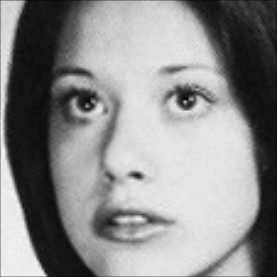
\includegraphics[width=0.75\linewidth]{most_bracco}
		\caption{Lorraine Bracco}
	\end{subfigure}%
	\begin{subfigure}{0.5\linewidth}
		\centering
		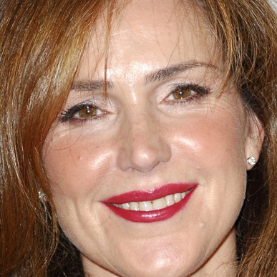
\includegraphics[width=0.75\linewidth]{most_gilpin}
		\caption{Peri Gilpin}
	\end{subfigure}\vspace{1em}
	\begin{subfigure}{0.5\linewidth}
		\centering
		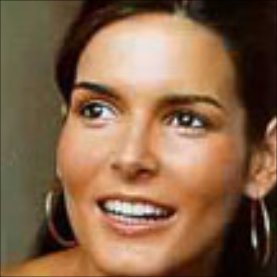
\includegraphics[width=0.75\linewidth]{most_harmon}
		\caption{Angie Harmon}
	\end{subfigure}%
	\begin{subfigure}{0.5\linewidth}
		\centering
		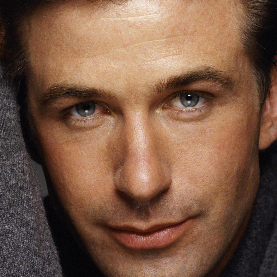
\includegraphics[width=0.75\linewidth]{most_baldwin}
		\caption{Alec Baldwin}
	\end{subfigure}\vspace{1em}
	\begin{subfigure}{0.5\linewidth}
		\centering
		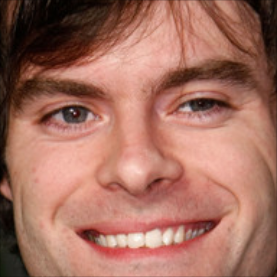
\includegraphics[width=0.75\linewidth]{most_hader}
		\caption{Bill Hader}
	\end{subfigure}%
	\begin{subfigure}{0.5\linewidth}
		\centering
		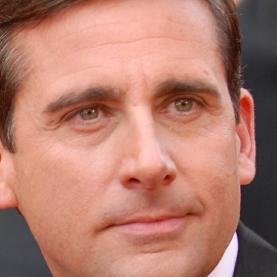
\includegraphics[width=0.75\linewidth]{most_carell}
		\caption{Steve Carell}
	\end{subfigure}
	\caption{Prototypical images associated with each actor, representing the least loss of any of the images in the dataset.}
	\label{fig:prototypical}
\end{figure}

\begin{figure}
	\begin{subfigure}[t]{0.33\linewidth}
		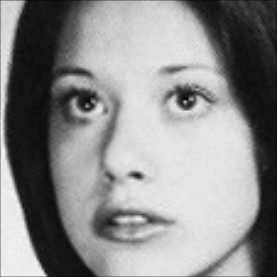
\includegraphics[width=\linewidth]{most_bracco}
		\caption{Lorraine Bracco}
	\end{subfigure}
	\begin{subfigure}[t]{0.33\linewidth}
		\includegraphics[width=\linewidth]{results/bracco_Vanilla_BP_color}
	\end{subfigure}
	\begin{subfigure}[t]{0.33\linewidth}
		\includegraphics[width=\linewidth]{results/bracco_Vanilla_BP_gray}
	\end{subfigure}\vspace{1em}
	\begin{subfigure}[t]{0.33\linewidth}
		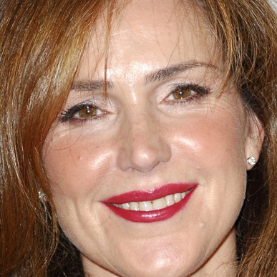
\includegraphics[width=\linewidth]{most_gilpin}
		\caption{Peri Gilpin}
	\end{subfigure}
	\begin{subfigure}[t]{0.33\linewidth}
		\includegraphics[width=\linewidth]{results/gilpin_Vanilla_BP_color}
	\end{subfigure}
	\begin{subfigure}[t]{0.33\linewidth}
		\includegraphics[width=\linewidth]{results/gilpin_Vanilla_BP_gray}
	\end{subfigure}\vspace{1em}
	\begin{subfigure}[t]{0.33\linewidth}
		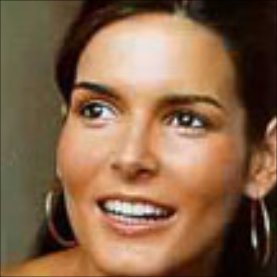
\includegraphics[width=\linewidth]{most_harmon}
		\caption{Angie Harmon}
	\end{subfigure}
	\begin{subfigure}[t]{0.33\linewidth}
		\includegraphics[width=\linewidth]{results/harmon_Vanilla_BP_color}
	\end{subfigure}
	\begin{subfigure}[t]{0.33\linewidth}
		\includegraphics[width=\linewidth]{results/harmon_Vanilla_BP_gray}
	\end{subfigure}\vspace{1em}
	\caption{Original image (left), gradients of the image produced via backpropagation (middle), and associated saliency map (right).}
\end{figure}
\begin{figure}
	\ContinuedFloat
	\begin{subfigure}[t]{0.33\linewidth}
		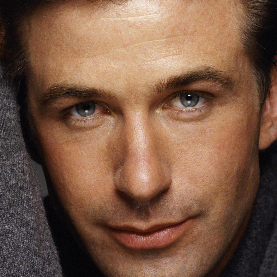
\includegraphics[width=\linewidth]{most_baldwin}
		\caption{Alec Baldwin}
	\end{subfigure}
	\begin{subfigure}[t]{0.33\linewidth}
		\includegraphics[width=\linewidth]{results/baldwin_Vanilla_BP_color}
	\end{subfigure}
	\begin{subfigure}[t]{0.33\linewidth}
		\includegraphics[width=\linewidth]{results/baldwin_Vanilla_BP_gray}
	\end{subfigure}\vspace{1em}
	\begin{subfigure}[t]{0.33\linewidth}
		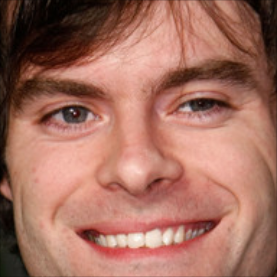
\includegraphics[width=\linewidth]{most_hader}
		\caption{Bill Hader}
	\end{subfigure}
	\begin{subfigure}[t]{0.33\linewidth}
		\includegraphics[width=\linewidth]{results/hader_Vanilla_BP_color}
	\end{subfigure}
	\begin{subfigure}[t]{0.33\linewidth}
		\includegraphics[width=\linewidth]{results/hader_Vanilla_BP_gray}
	\end{subfigure}\vspace{1em}
	\begin{subfigure}[t]{0.33\linewidth}
		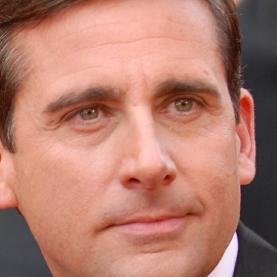
\includegraphics[width=\linewidth]{most_carell}
		\caption{Steve Carell}
	\end{subfigure}
	\begin{subfigure}[t]{0.33\linewidth}
		\includegraphics[width=\linewidth]{results/carell_Vanilla_BP_color}
	\end{subfigure}
	\begin{subfigure}[t]{0.33\linewidth}
		\includegraphics[width=\linewidth]{results/carell_Vanilla_BP_gray}
	\end{subfigure}
	\caption{(Cont.) Original image (left), gradients of the image produced via backpropagation (middle), and associated saliency map (right).}
	\label{fig:vanilla backpropagation}
\end{figure}

\begin{figure}
	\begin{subfigure}[t]{0.33\linewidth}
		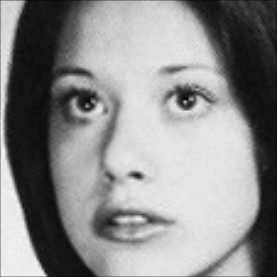
\includegraphics[width=\linewidth]{most_bracco}
		\caption{Lorraine Bracco}
	\end{subfigure}
	\begin{subfigure}[t]{0.33\linewidth}
		\includegraphics[width=\linewidth]{results/bracco_Guided_BP_colour}
	\end{subfigure}
	\begin{subfigure}[t]{0.33\linewidth}
		\includegraphics[width=\linewidth]{results/bracco_Guided_BP_gray}
	\end{subfigure}\vspace{1em}
	\begin{subfigure}[t]{0.33\linewidth}
		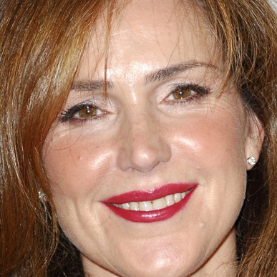
\includegraphics[width=\linewidth]{most_gilpin}
		\caption{Peri Gilpin}
	\end{subfigure}
	\begin{subfigure}[t]{0.33\linewidth}
		\includegraphics[width=\linewidth]{results/gilpin_Guided_BP_colour}
	\end{subfigure}
	\begin{subfigure}[t]{0.33\linewidth}
		\includegraphics[width=\linewidth]{results/gilpin_Guided_BP_gray}
	\end{subfigure}\vspace{1em}
	\begin{subfigure}[t]{0.33\linewidth}
		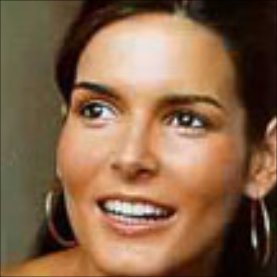
\includegraphics[width=\linewidth]{most_harmon}
		\caption{Angie Harmon}
	\end{subfigure}
	\begin{subfigure}[t]{0.33\linewidth}
		\includegraphics[width=\linewidth]{results/harmon_Guided_BP_colour}
	\end{subfigure}
	\begin{subfigure}[t]{0.33\linewidth}
		\includegraphics[width=\linewidth]{results/harmon_Guided_BP_gray}
	\end{subfigure}\vspace{1em}
	\caption{Original image (left), gradients of the image produced via guided backpropagation (middle), and associated saliency map (right).}
\end{figure}
\begin{figure}
	\ContinuedFloat
	\begin{subfigure}[t]{0.33\linewidth}
		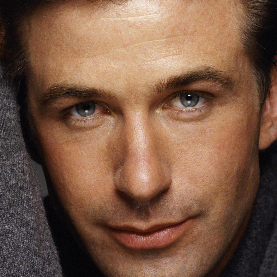
\includegraphics[width=\linewidth]{most_baldwin}
		\caption{Alec Baldwin}
	\end{subfigure}
	\begin{subfigure}[t]{0.33\linewidth}
		\includegraphics[width=\linewidth]{results/baldwin_Guided_BP_colour}
	\end{subfigure}
	\begin{subfigure}[t]{0.33\linewidth}
		\includegraphics[width=\linewidth]{results/baldwin_Guided_BP_gray}
	\end{subfigure}\vspace{1em}
	\begin{subfigure}[t]{0.33\linewidth}
		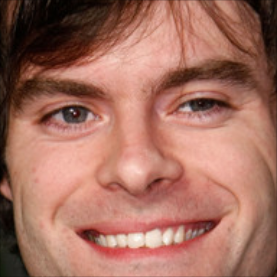
\includegraphics[width=\linewidth]{most_hader}
		\caption{Bill Hader}
	\end{subfigure}
	\begin{subfigure}[t]{0.33\linewidth}
		\includegraphics[width=\linewidth]{results/hader_Guided_BP_colour}
	\end{subfigure}
	\begin{subfigure}[t]{0.33\linewidth}
		\includegraphics[width=\linewidth]{results/hader_Guided_BP_gray}
	\end{subfigure}\vspace{1em}
	\begin{subfigure}[t]{0.33\linewidth}
		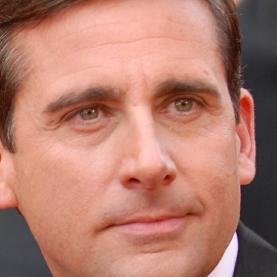
\includegraphics[width=\linewidth]{most_carell}
		\caption{Steve Carell}
	\end{subfigure}
	\begin{subfigure}[t]{0.33\linewidth}
		\includegraphics[width=\linewidth]{results/carell_Guided_BP_colour}
	\end{subfigure}
	\begin{subfigure}[t]{0.33\linewidth}
		\includegraphics[width=\linewidth]{results/carell_Guided_BP_gray}
	\end{subfigure}
	\caption{(Cont.) Original image (left), gradients of the image produced via guided backpropagation (middle), and associated saliency map (right).}
	\label{fig:guided backpropagation}
\end{figure}

\begin{figure}
	\begin{subfigure}[t]{0.33\linewidth}
		\includegraphics[width=\linewidth]{results/bracco_layer0_Cam_On_Image}
		\caption{Lorraine Bracco}
	\end{subfigure}
	\begin{subfigure}[t]{0.33\linewidth}
		\includegraphics[width=\linewidth]{results/bracco_layer3_Cam_On_Image}
	\end{subfigure}
	\begin{subfigure}[t]{0.33\linewidth}
		\includegraphics[width=\linewidth]{results/bracco_layer9_Cam_On_Image}
	\end{subfigure}\vspace{1em}
	\begin{subfigure}[t]{0.33\linewidth}
		\includegraphics[width=\linewidth]{results/gilpin_layer0_Cam_On_Image}
		\caption{Peri Gilpin}
	\end{subfigure}
	\begin{subfigure}[t]{0.33\linewidth}
		\includegraphics[width=\linewidth]{results/gilpin_layer3_Cam_On_Image}
	\end{subfigure}
	\begin{subfigure}[t]{0.33\linewidth}
		\includegraphics[width=\linewidth]{results/gilpin_layer9_Cam_On_Image}
	\end{subfigure}\vspace{1em}
	\begin{subfigure}[t]{0.33\linewidth}
		\includegraphics[width=\linewidth]{results/harmon_layer0_Cam_On_Image}
		\caption{Angie Harmon}
	\end{subfigure}
	\begin{subfigure}[t]{0.33\linewidth}
		\includegraphics[width=\linewidth]{results/harmon_layer3_Cam_On_Image}
	\end{subfigure}
	\begin{subfigure}[t]{0.33\linewidth}
		\includegraphics[width=\linewidth]{results/harmon_layer9_Cam_On_Image}
	\end{subfigure}\vspace{1em}
	\caption{GradCAM after first convulutional layer (left), GradCAM after second convulutional layer (middle), and GradCAM at layer before fully connected layer (right).}
\end{figure}
\begin{figure}
	\ContinuedFloat
	\begin{subfigure}[t]{0.33\linewidth}
		\includegraphics[width=\linewidth]{results/baldwin_layer0_Cam_On_Image}
		\caption{Alec Baldwin}
	\end{subfigure}
	\begin{subfigure}[t]{0.33\linewidth}
		\includegraphics[width=\linewidth]{results/baldwin_layer3_Cam_On_Image}
	\end{subfigure}
	\begin{subfigure}[t]{0.33\linewidth}
		\includegraphics[width=\linewidth]{results/baldwin_layer9_Cam_On_Image}
	\end{subfigure}\vspace{1em}
	\begin{subfigure}[t]{0.33\linewidth}
		\includegraphics[width=\linewidth]{results/hader_layer0_Cam_On_Image}
		\caption{Bill Hader}
	\end{subfigure}
	\begin{subfigure}[t]{0.33\linewidth}
		\includegraphics[width=\linewidth]{results/hader_layer3_Cam_On_Image}
	\end{subfigure}
	\begin{subfigure}[t]{0.33\linewidth}
		\includegraphics[width=\linewidth]{results/hader_layer9_Cam_On_Image}
	\end{subfigure}\vspace{1em}
	\begin{subfigure}[t]{0.33\linewidth}
		\includegraphics[width=\linewidth]{results/carell_layer0_Cam_On_Image}
		\caption{Steve Carell}
	\end{subfigure}
	\begin{subfigure}[t]{0.33\linewidth}
		\includegraphics[width=\linewidth]{results/carell_layer3_Cam_On_Image}
	\end{subfigure}
	\begin{subfigure}[t]{0.33\linewidth}
		\includegraphics[width=\linewidth]{results/carell_layer9_Cam_On_Image}
	\end{subfigure}
	\caption{(Cont.) GradCAM after first convulutional layer (left), GradCAM after second convulutional layer (middle), and GradCAM at layer before fully connected layer (right).}
	\label{fig:gradcam}
\end{figure}

\begin{figure}
	\begin{subfigure}{0.5\linewidth}
		\centering
		\includegraphics[width=0.75\linewidth]{generated/bracco/braccoc_specific_iteration_149}
		\caption{Lorraine Bracco}
	\end{subfigure}%
	\begin{subfigure}{0.5\linewidth}
		\centering
		\includegraphics[width=0.75\linewidth]{generated/gilpin/gilpinc_specific_iteration_149}
		\caption{Peri Gilpin}
	\end{subfigure}\vspace{1em}
	\begin{subfigure}{0.5\linewidth}
		\centering
		\includegraphics[width=0.75\linewidth]{generated/harmon/harmonc_specific_iteration_149}
		\caption{Angie Harmon}
	\end{subfigure}%
	\begin{subfigure}{0.5\linewidth}
		\centering
		\includegraphics[width=0.75\linewidth]{generated/baldwin/baldwinc_specific_iteration_149}
		\caption{Alec Baldwin}
	\end{subfigure}\vspace{1em}
	\begin{subfigure}{0.5\linewidth}
		\centering
		\includegraphics[width=0.75\linewidth]{generated/hader/haderc_specific_iteration_149}
		\caption{Bill Hader}
	\end{subfigure}%
	\begin{subfigure}{0.5\linewidth}
		\centering
		\includegraphics[width=0.75\linewidth]{generated/carell/carellc_specific_iteration_149}
		\caption{Steve Carell}
	\end{subfigure}
	\caption{Results of class specific image generation after 150 iterations with no regularization.}
	\label{fig:class-spec}
\end{figure}

\clearpage

\printbibliography




\end{document}